\chapter{Results of the H2Mu search} \label{chp:hmm_results}

The analysis in the VH category is combined with those in the \ggH, \qqH, and \ttH categories.
Figure~\ref{fig:sum_cats_comp} summarizes the expected signal composition in all sub-categories of the \hmm analysis.
Figure~\ref{fig:sum_cats_SB} summarizes the expected $S/(S+B)$ and $S/\sqrt{B}$ in all sub-categories,
in which the signal and background yields are calculated by integrating the expectations within the FWHM range of the signal peak for the \ggH, \VH, and \ttH sub-categories,
while for the \qqH category the considered mass range is $115 \GeV < \mmm < 135 \GeV$.
For both figures, the mass of the Higgs boson is expected at \mh = 125.38~\GeV~\cite{2020135425},
which is the most precise measurement of the Higgs mass up to date.

\begin{figure*}[!htb]
    \centering
    \captionsetup{justification=justified}
    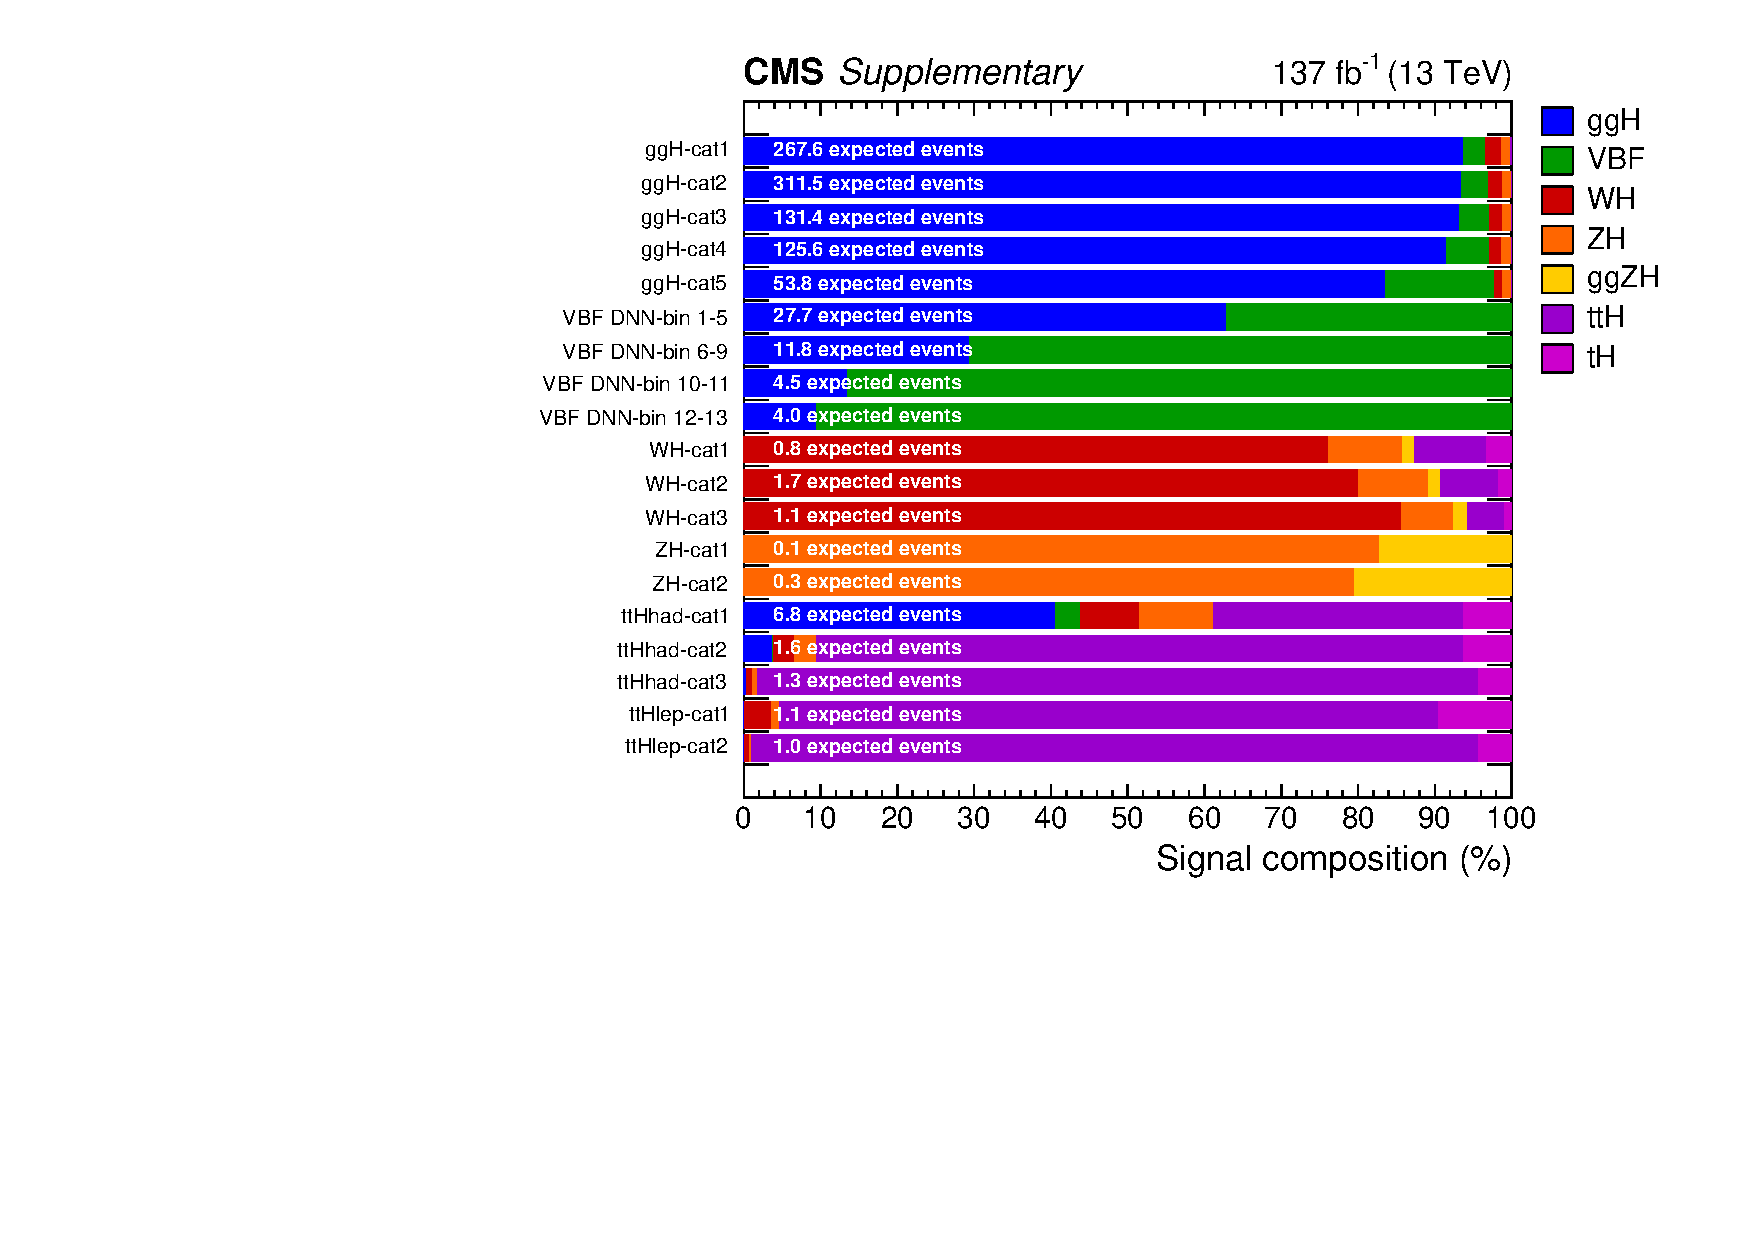
\includegraphics[width=0.80\textwidth]{pics/results/sig_composition.pdf}
    \caption{Expected fraction of signal events per production mode in the different sub-categories for \mh = 125.38~\GeV.
             The tH contribution is defined as the sum of \tHq and \tHW processes.
             Plot taken from Ref.~\cite{Sirunyan_2021}.}
    \label{fig:sum_cats_comp}
\end{figure*}

\begin{figure*}[!htb]
    \centering
    \captionsetup{justification=justified}
    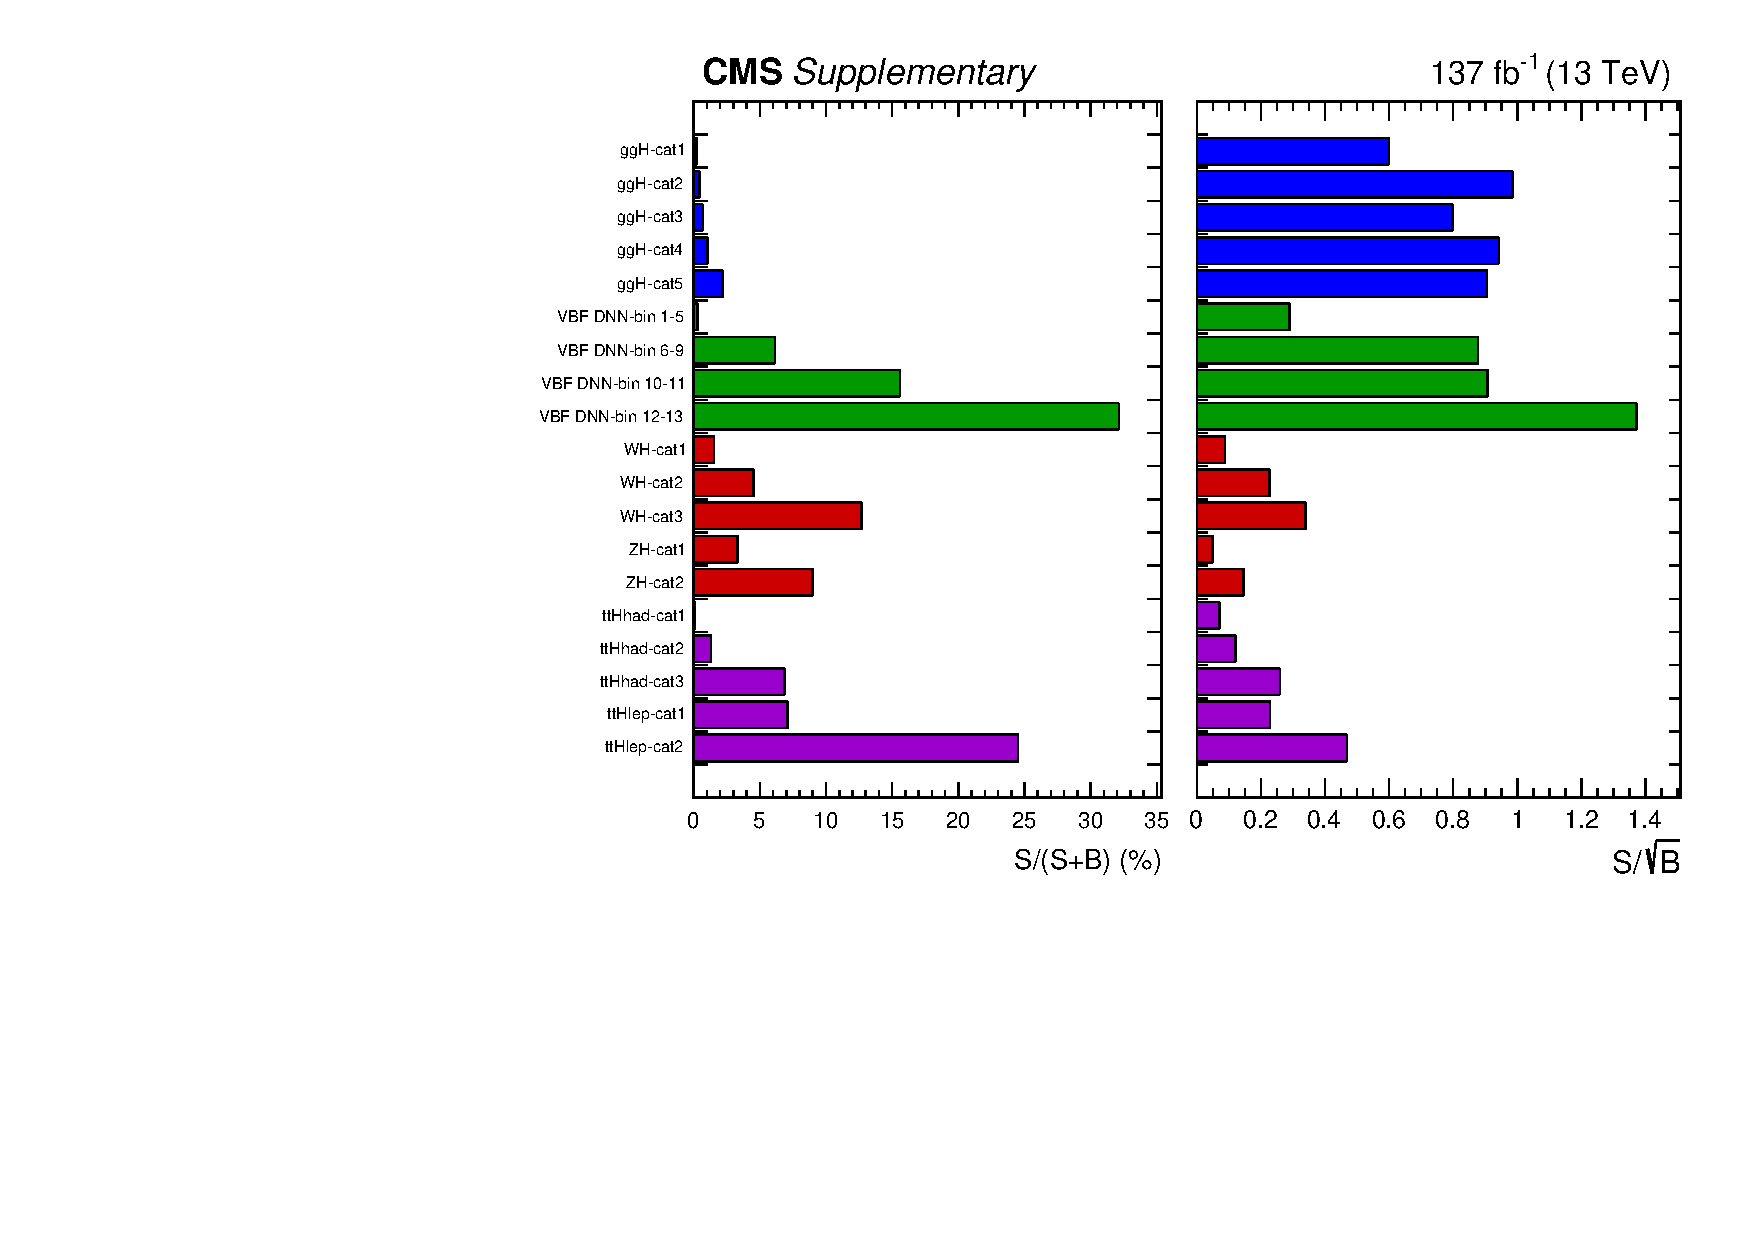
\includegraphics[width=0.80\textwidth]{pics/results/purity_signif.pdf}
    \caption{Expected $S/(S+B)$ and $S/\sqrt{B}$ in different sub-categories, 
             where $S$ and $B$ indicate the number of expect signal and background events, respectively.
             Plot taken from Ref.~\cite{Sirunyan_2021}.}
    \label{fig:sum_cats_SB}
\end{figure*}

The individual signal strength modifier from each category is summarized in Figure~\ref{fig:sum_sig_strength},
with the Higgs signal expected at \mh = 125.38~\GeV.
A combined fit is performed across all categories with one common signal strength modifier, 
whose best fit value is $\hat{\mu} = 1.19^{+0.41}_{-0.40} \text{(stat)}^{+0.17}_{-0.16} \text{(syst)}$, 
shown in the plot as the solid red line.

\begin{figure*}[!htb]
    \centering
    \captionsetup{justification=justified}
    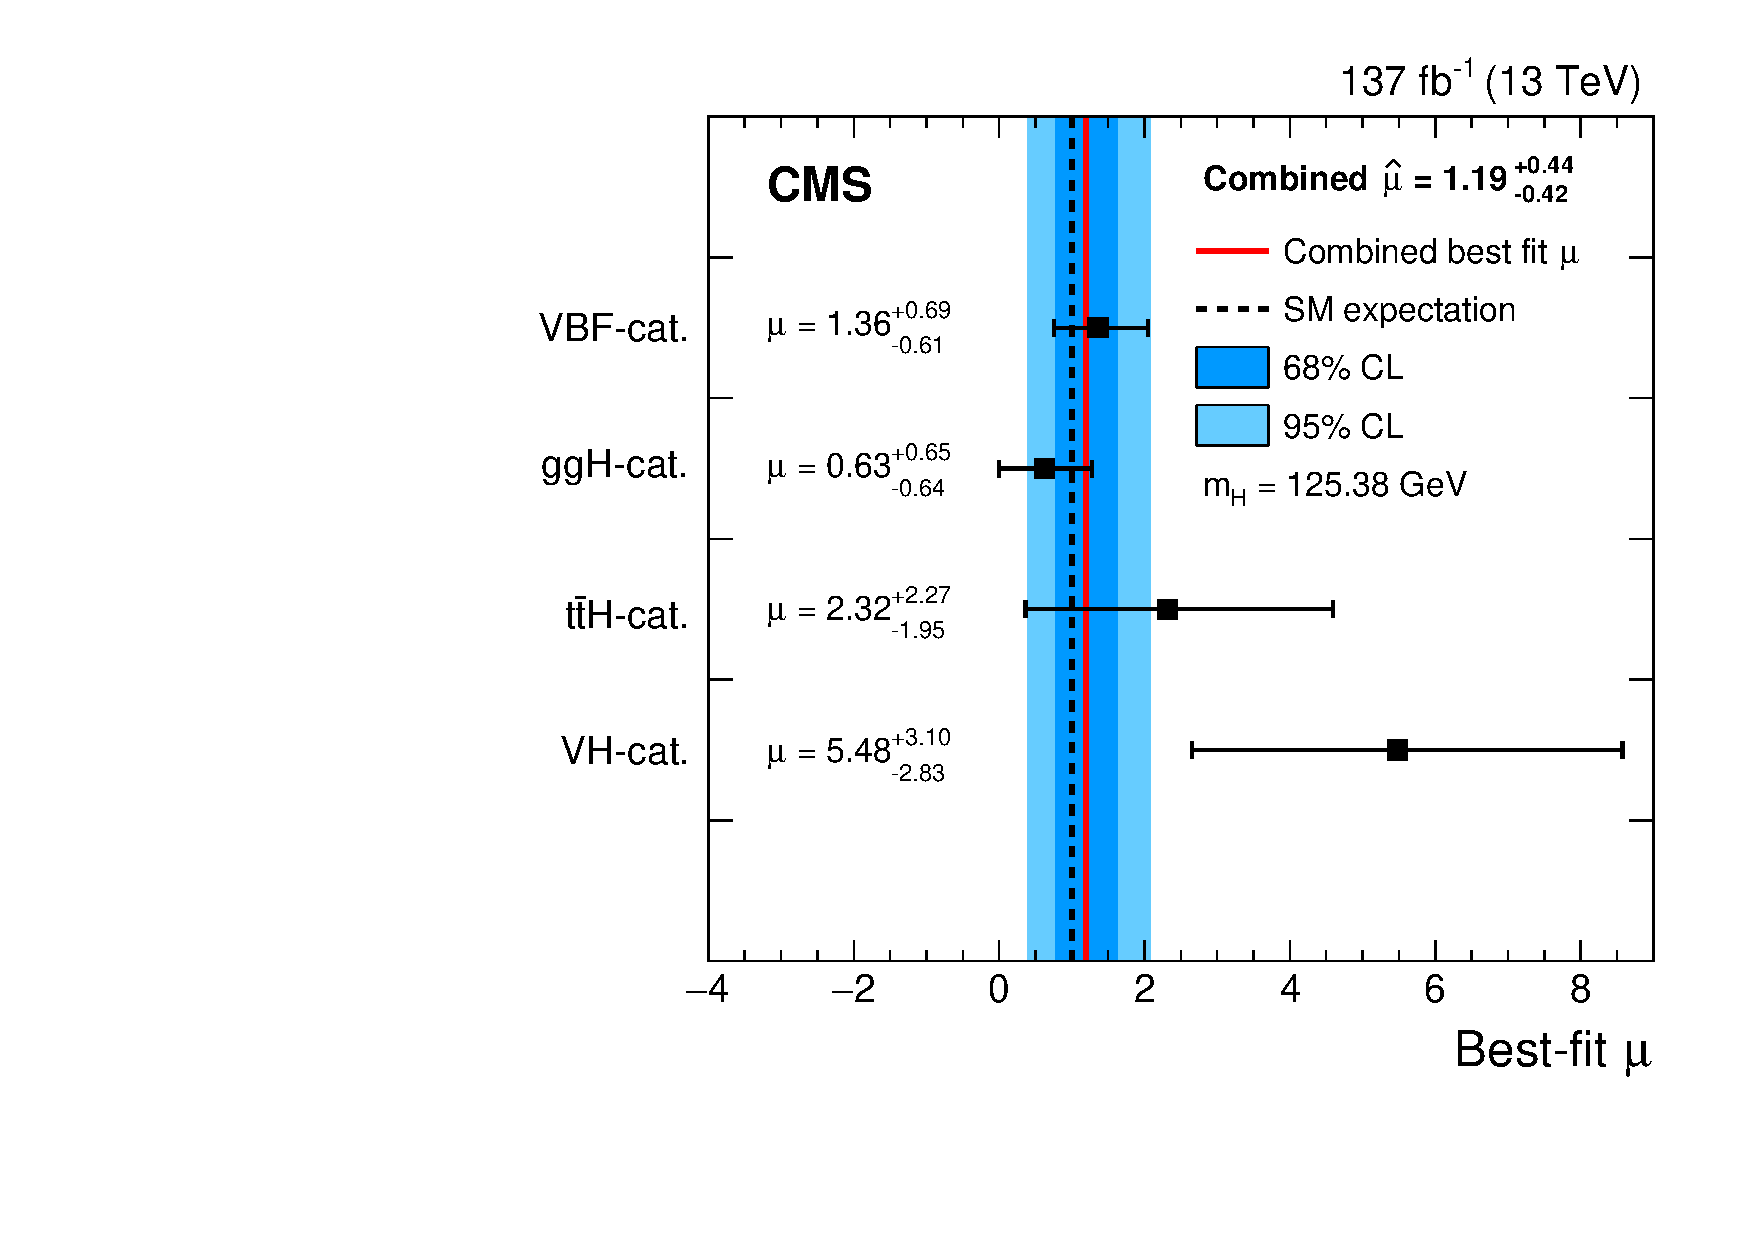
\includegraphics[width=0.60\textwidth]{pics/results/sig_strength.pdf}
    \caption{Signal strength modifiers measured for \mh = 125.38~\GeV in each production category (black points) 
             are compared to the result of the combined fit (solid red line) and the SM expectation (dashed gray line).
             Plot taken from Ref.~\cite{Sirunyan_2021}. }
    \label{fig:sum_sig_strength}
\end{figure*}

The statistical significance of the presence of the signal is tested against the null hypothesis,
in which no signal is expected and the observed distribution is raised by the statistical fluctuation in the background.
A scan of p-value is performed across the mass range of $120 \GeV< \mh < 130 \GeV$, 
which quantifies the probability for the background to produce a fluctuation larger than the apparent signal observed in the search region.
Figure~\ref{fig:p_value_scan} shows the observed and expected (with a signal at 125.38~\GeV and $\mu = 1$) p-values for individual categories as well as the overall combination.
The overall observed (expected for $\mu = 1$) significance at \mh = 125.38~\GeV of the incompatibility with the background-only hypothesis is 3.0~(2.5) standard deviations,
while the observed (expected for $\mu = 0$) upper limit of the signal strength at the 95\% confidence level is 1.9~(0.8) times the SM expectation.
This result makes the most sensitive measurement of the \hmm decay rate, establishing the first evidence of the Higgs boson decay to fermions of the second generation. 

\begin{figure*}[!htb]
    \centering
    \captionsetup{justification=justified}
    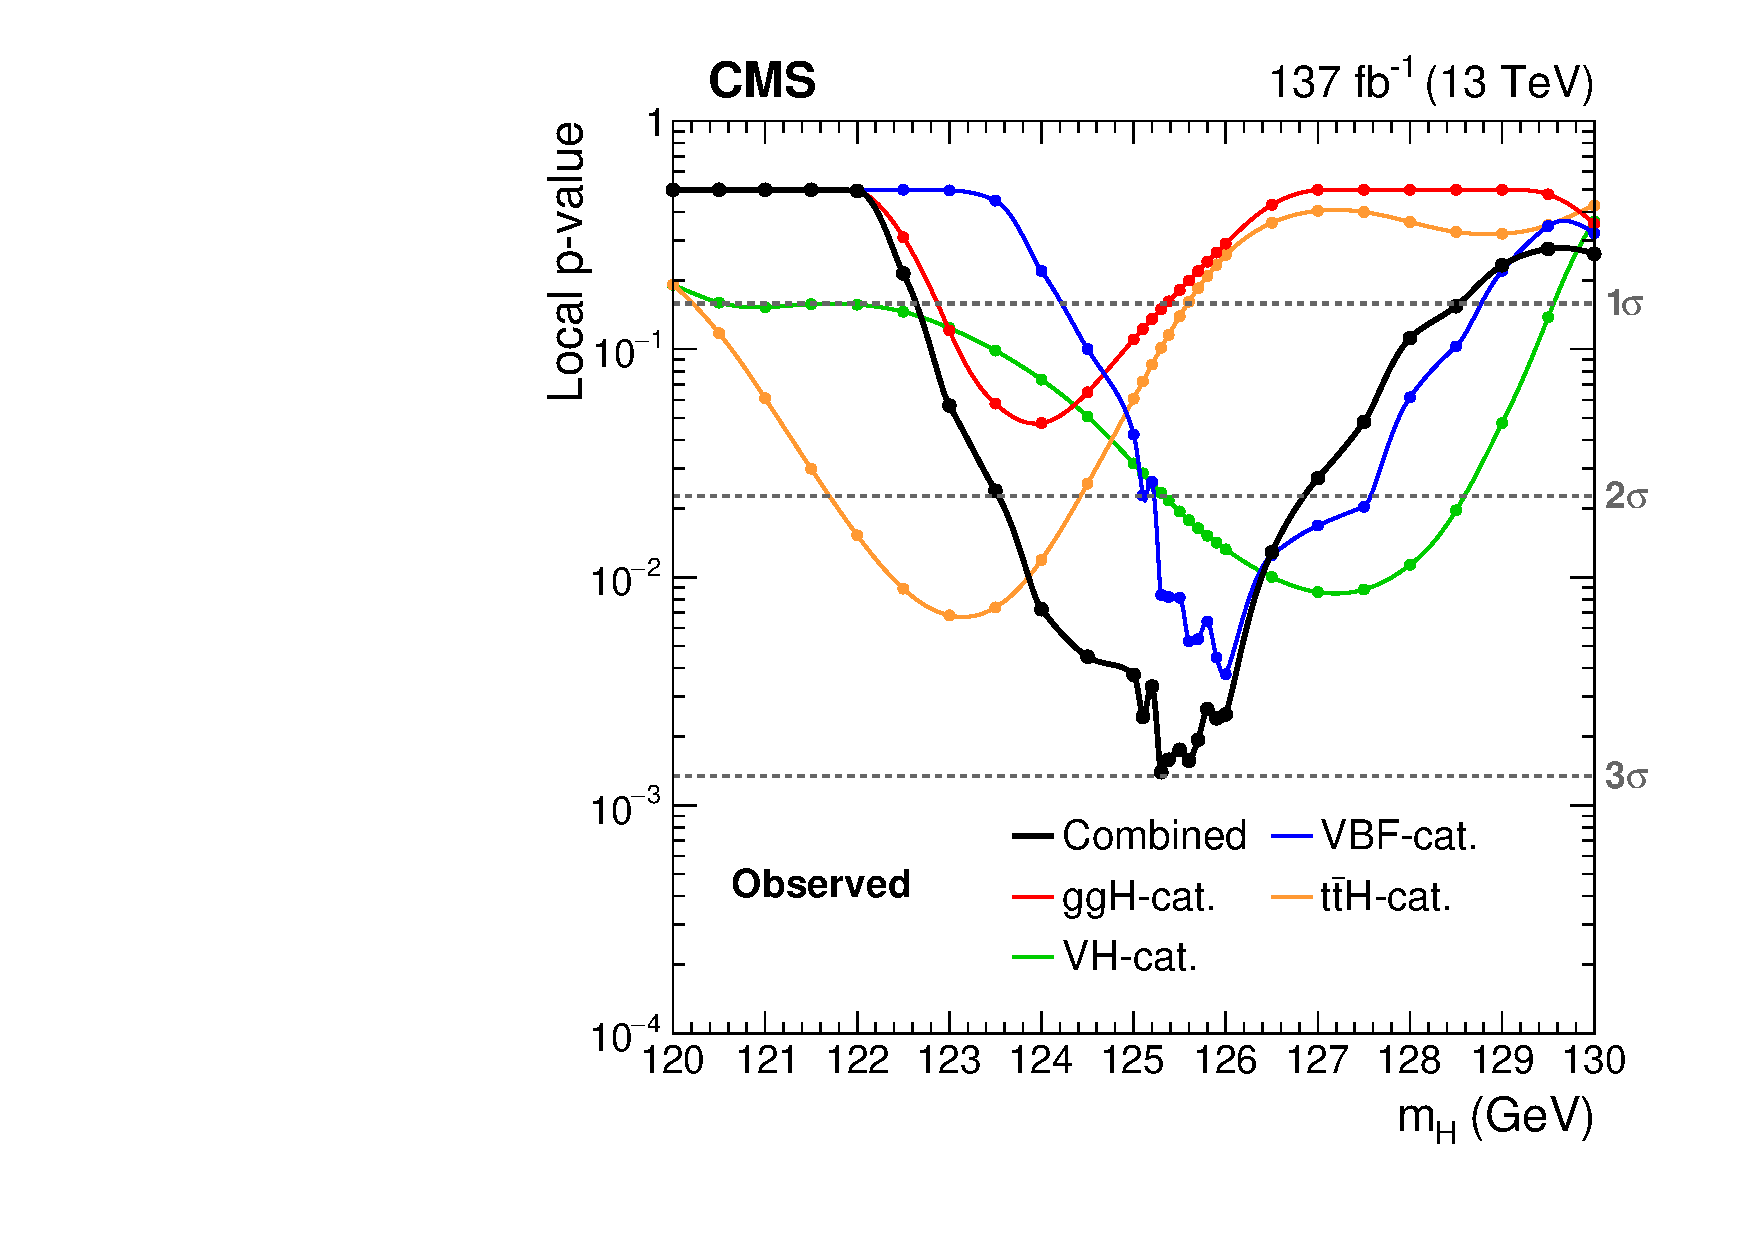
\includegraphics[width=0.45\textwidth]{pics/results/p-value_obs.pdf}
    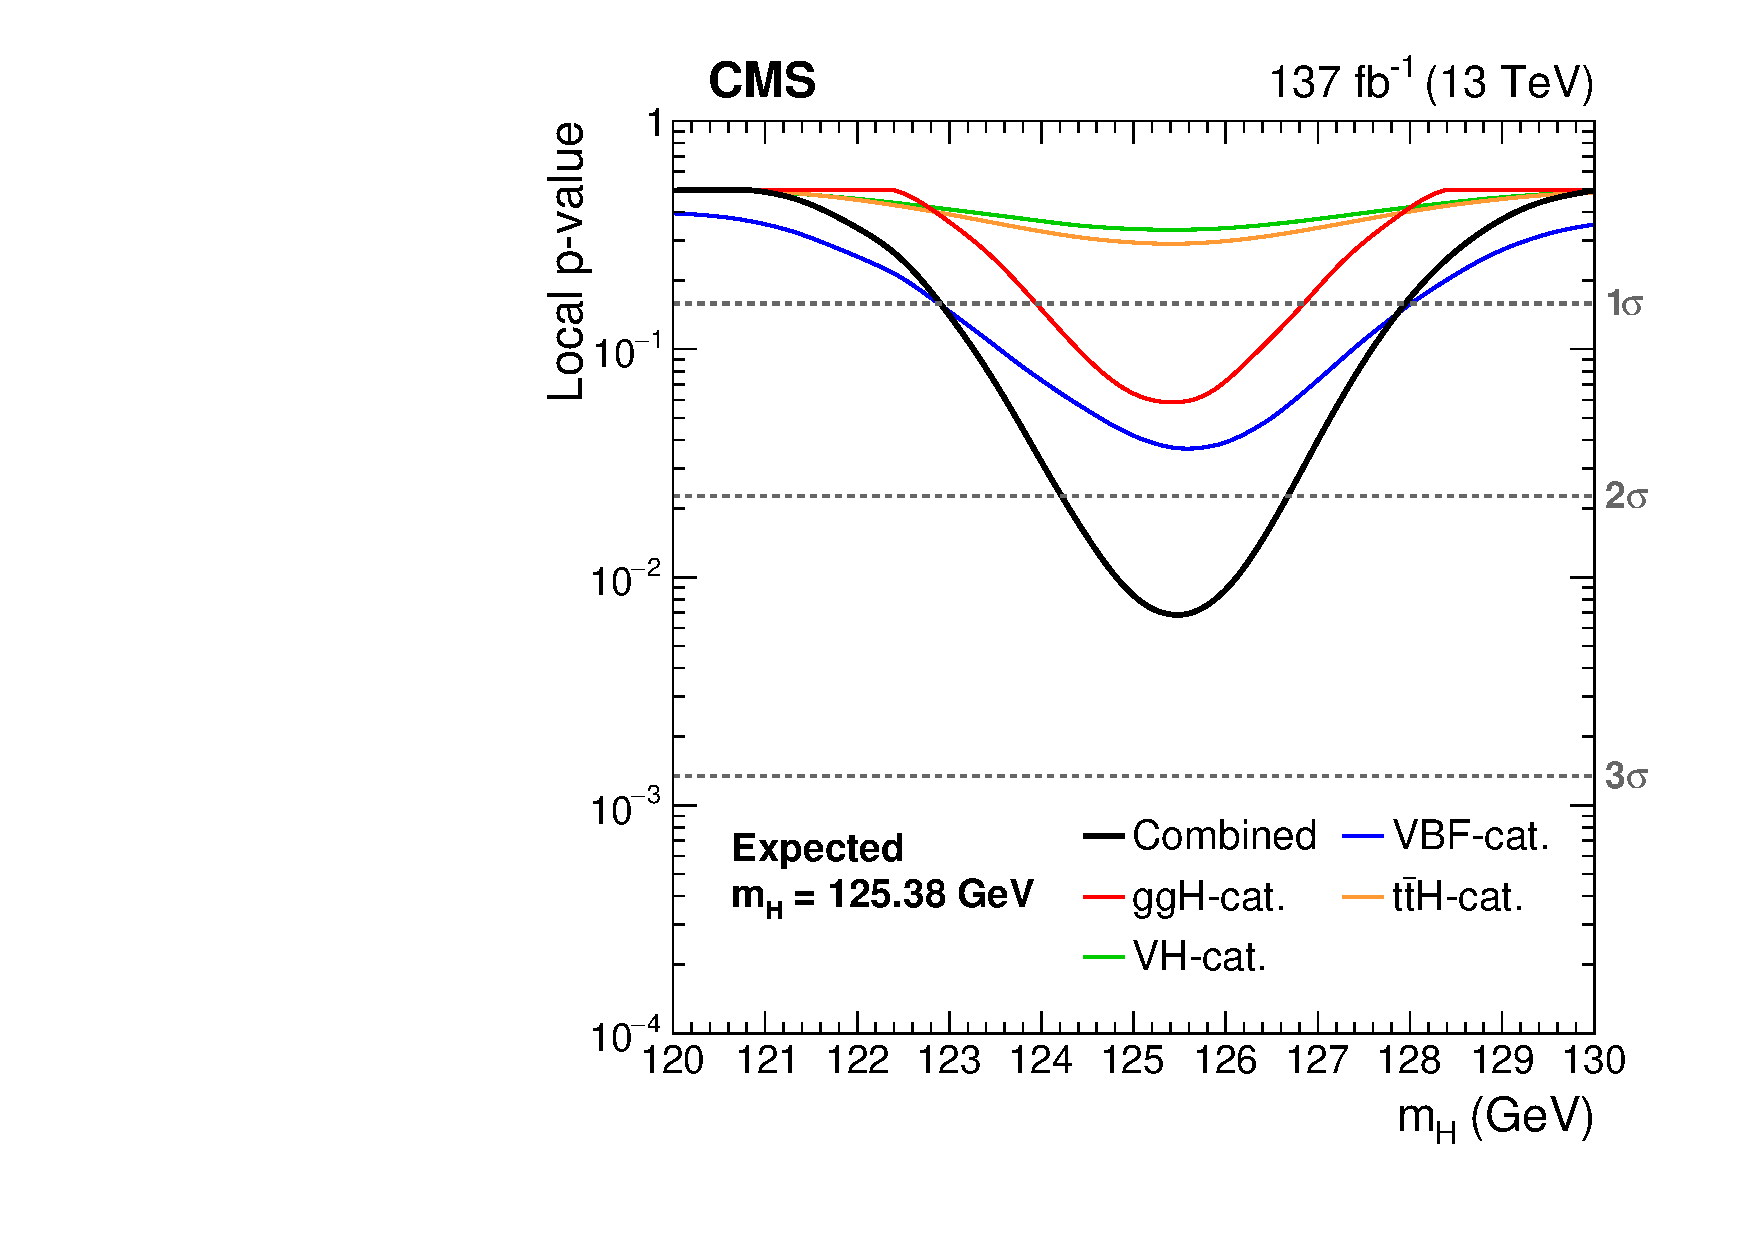
\includegraphics[width=0.45\textwidth]{pics/results/p-value_exp.pdf}
    \caption{The local p-values as a function of different \mh hypotheses, 
             for each individual categories as well as the overall combination.
             The left plot shows the observed p-values, 
             each solid marker indicating a mass point for which the observed p-values are computed.
             The right plot shows the expected p-values calculated using the background estimate from the S+B fit 
             and injecting a signal with \mh = 125.38~\GeV and $\mu = 1$.
             Plot taken from Ref.~\cite{Sirunyan_2021}.}
    \label{fig:p_value_scan}
\end{figure*}

Finally, the measurement of the \hmm decay rate also provides the measurement on the coupling strength between the Higgs boson and the muon.
The coupling strength is evaluated in the $\kappa$-framework \cite{Heinemeyer:2013tqa} and the fit result is shown in Figure~\ref{fig:kappa_scan}.
The best fit value for $\kappa_{\mu}$ is 1.07 and the corresponding observed 68\% confidence interval is $0.85 < \kappa_{\mu} < 1.29$.
This result is furthermore combined with the measurements of the Higgs boson couplings to other particles presented in Ref.~\cite{Sirunyan:2640611},
which is based on $pp$ collision data recorded by CMS in 2016, corresponding to an integrated luminosity of 35.9~\invfb.
As a result, Figure~\ref{fig:higgs_2016} is updated to Figure~\ref{fig:higgs_coupling_new}, providing the best estimated of 
the six coupling strength modifiers for the Higgs boson coupling to leptons, quarks, and gauge bosons up to date.

\begin{figure*}[!htb]
    \centering
    \captionsetup{justification=justified}
    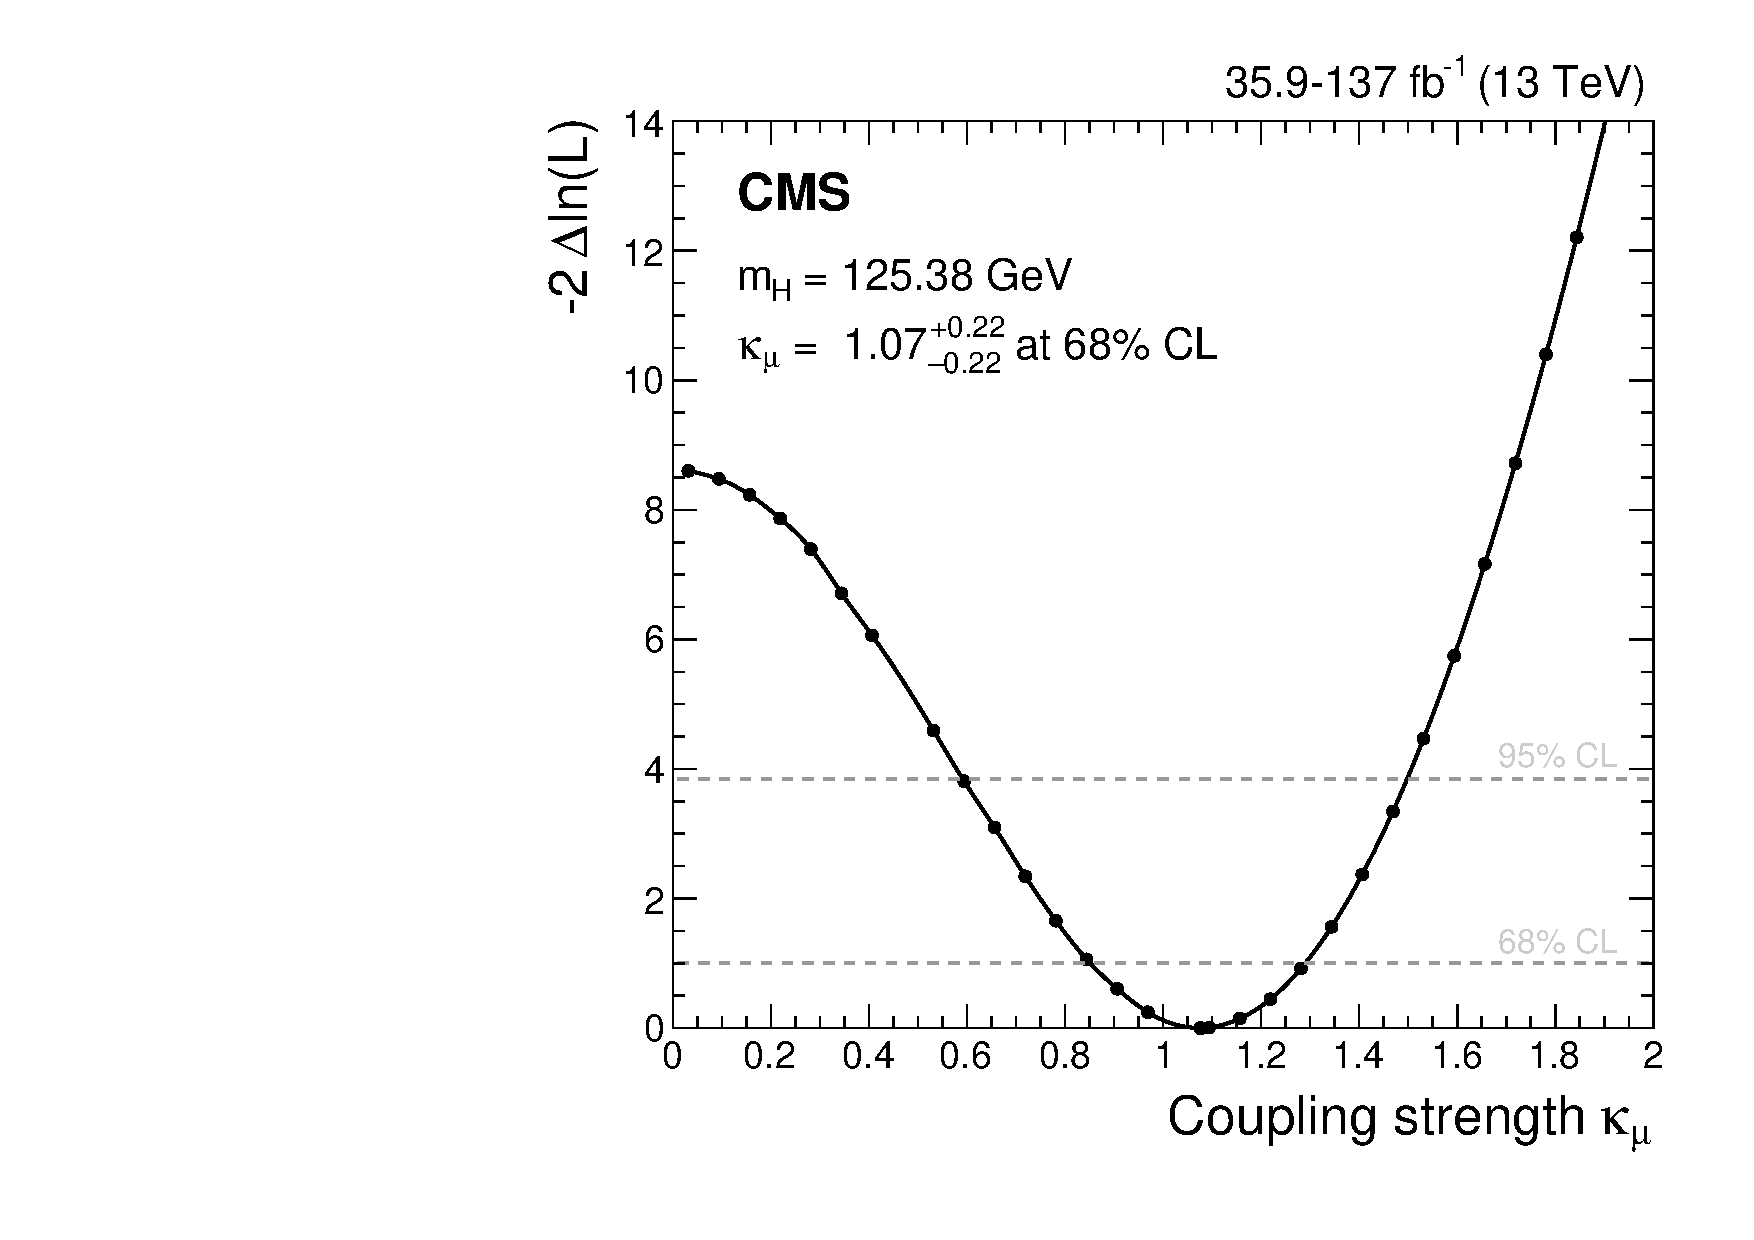
\includegraphics[width=0.60\textwidth]{pics/results/kappa_mu.pdf}
    \caption{The observed profile likelihood ratio as a function of $\kappa_{\mu}$ for \mh = 125.38~\GeV.
             Plot taken from Ref.~\cite{Sirunyan_2021}. }
    \label{fig:kappa_scan}
\end{figure*}

\begin{figure*}[!htb]
    \centering
    \captionsetup{justification=justified}
    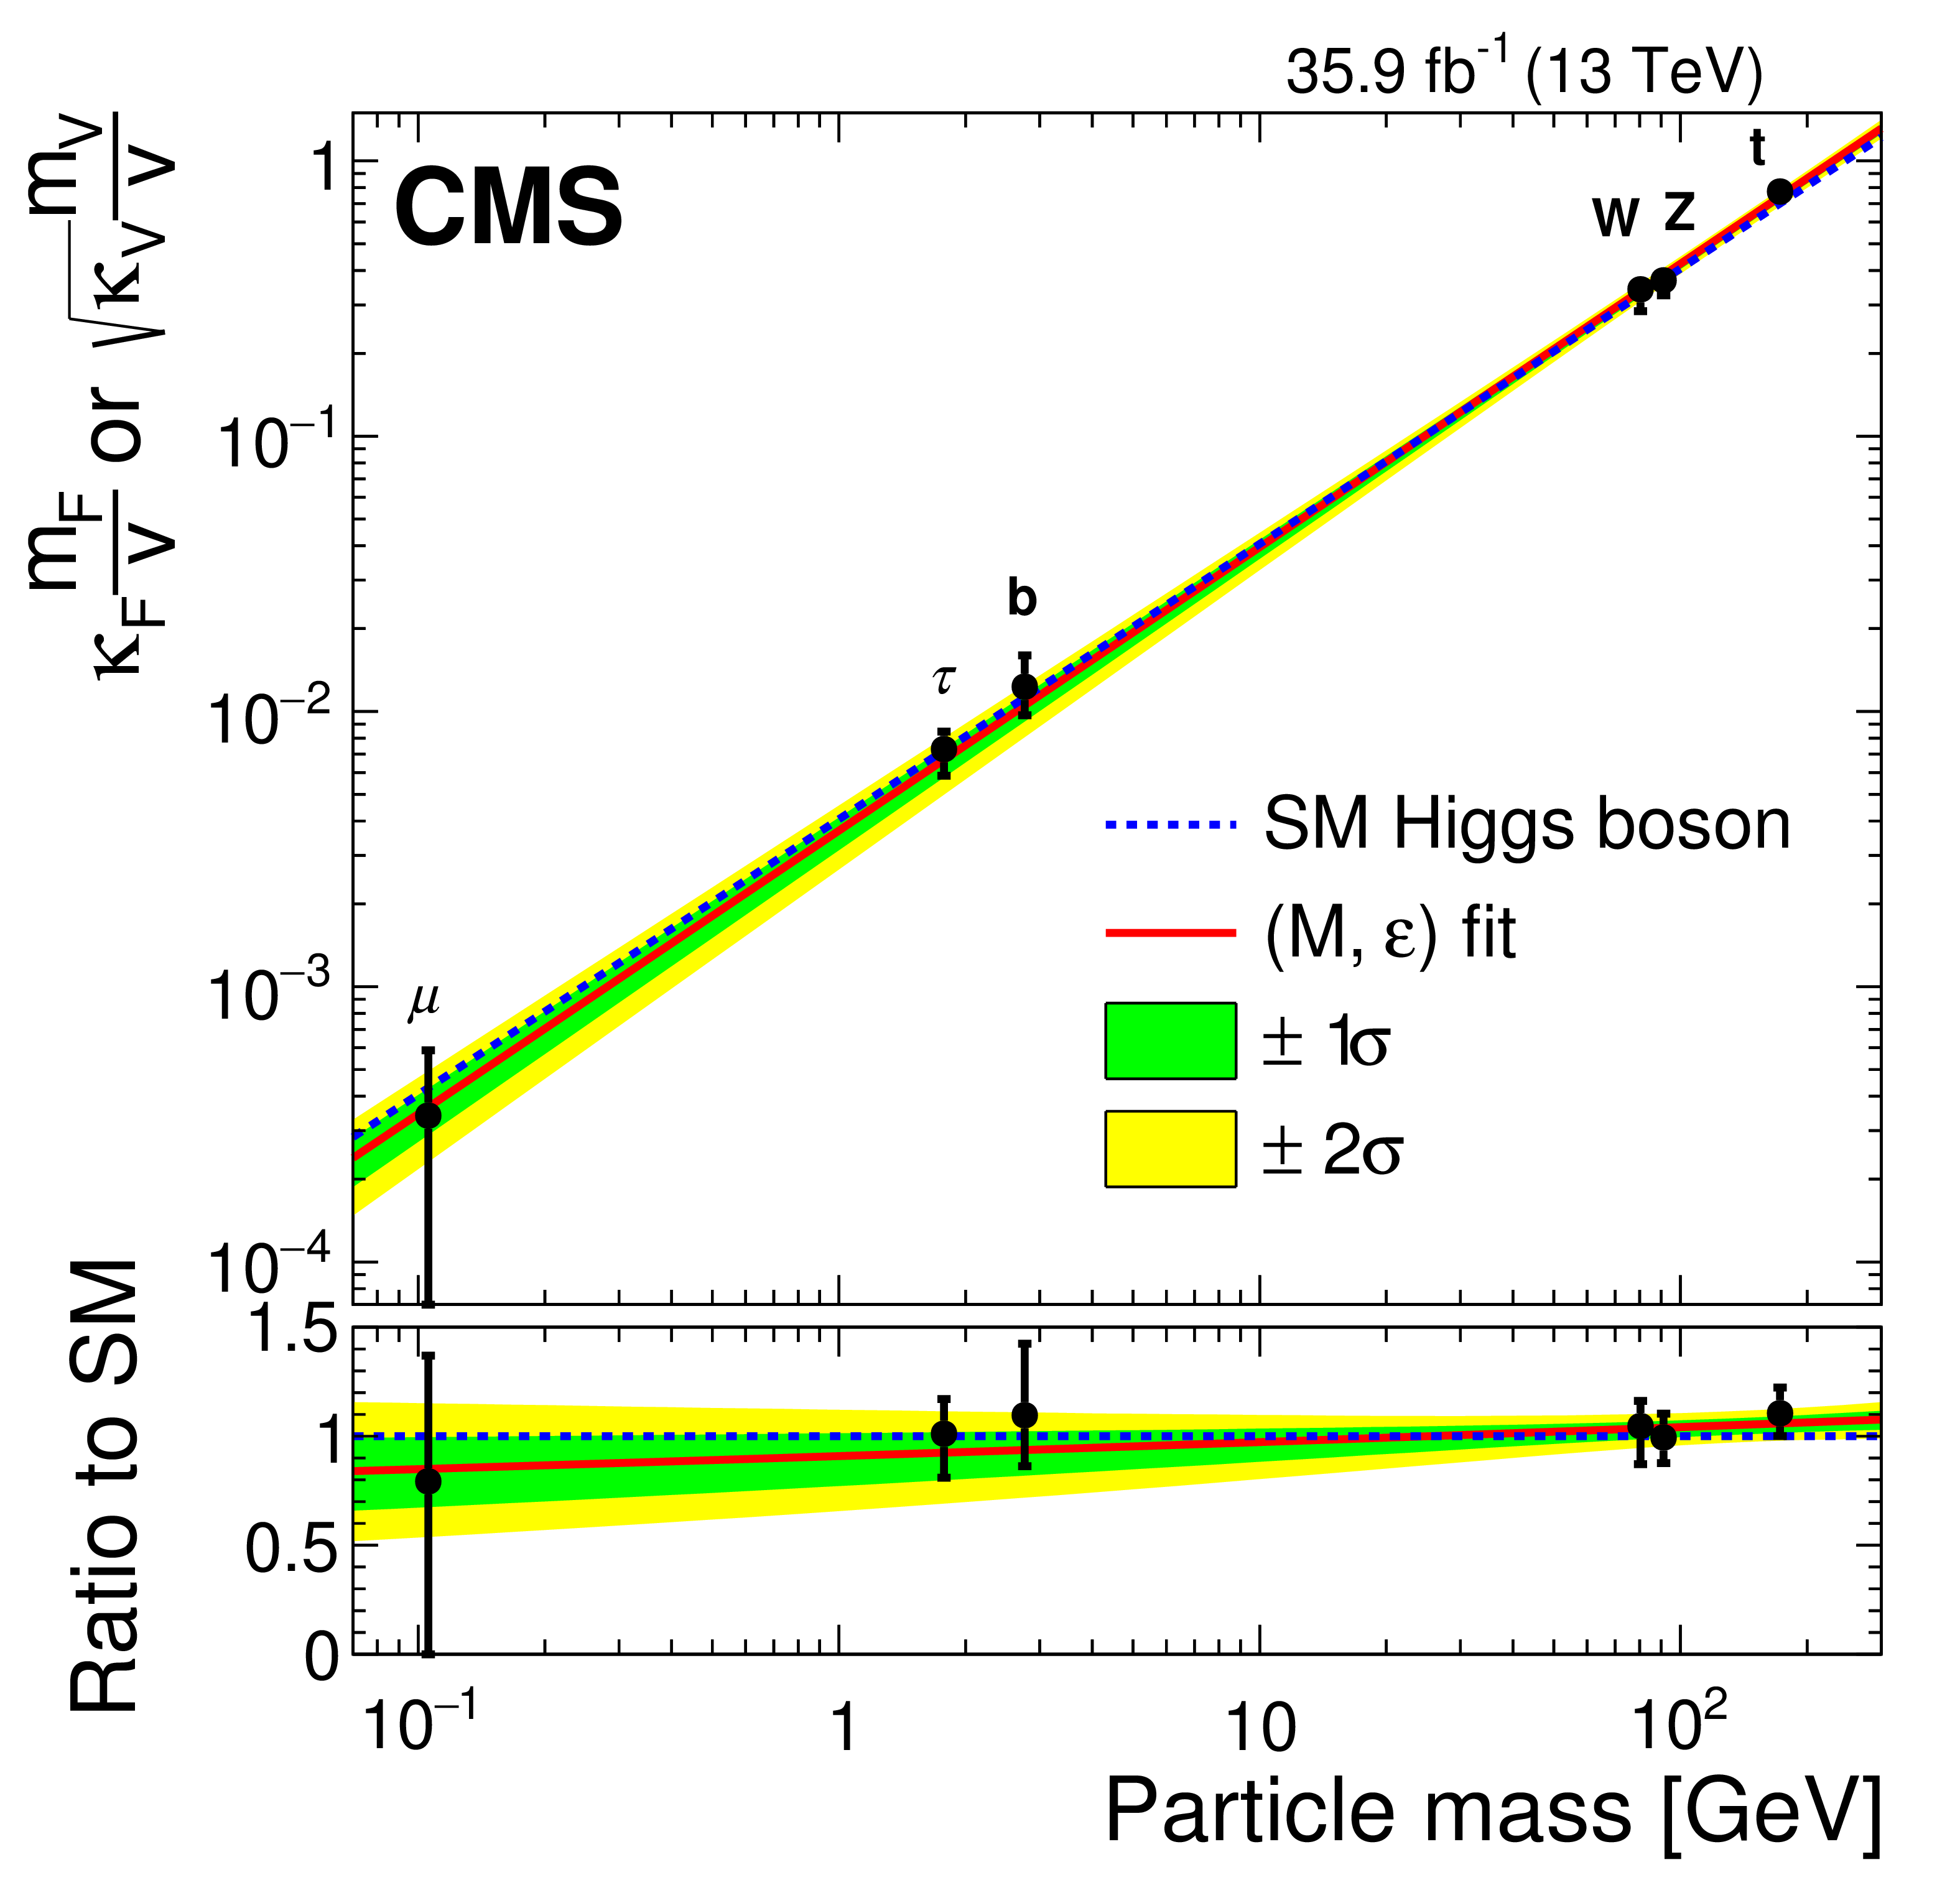
\includegraphics[width=0.45\textwidth]{pics/Intro/higgs_coupling_2016.png}
    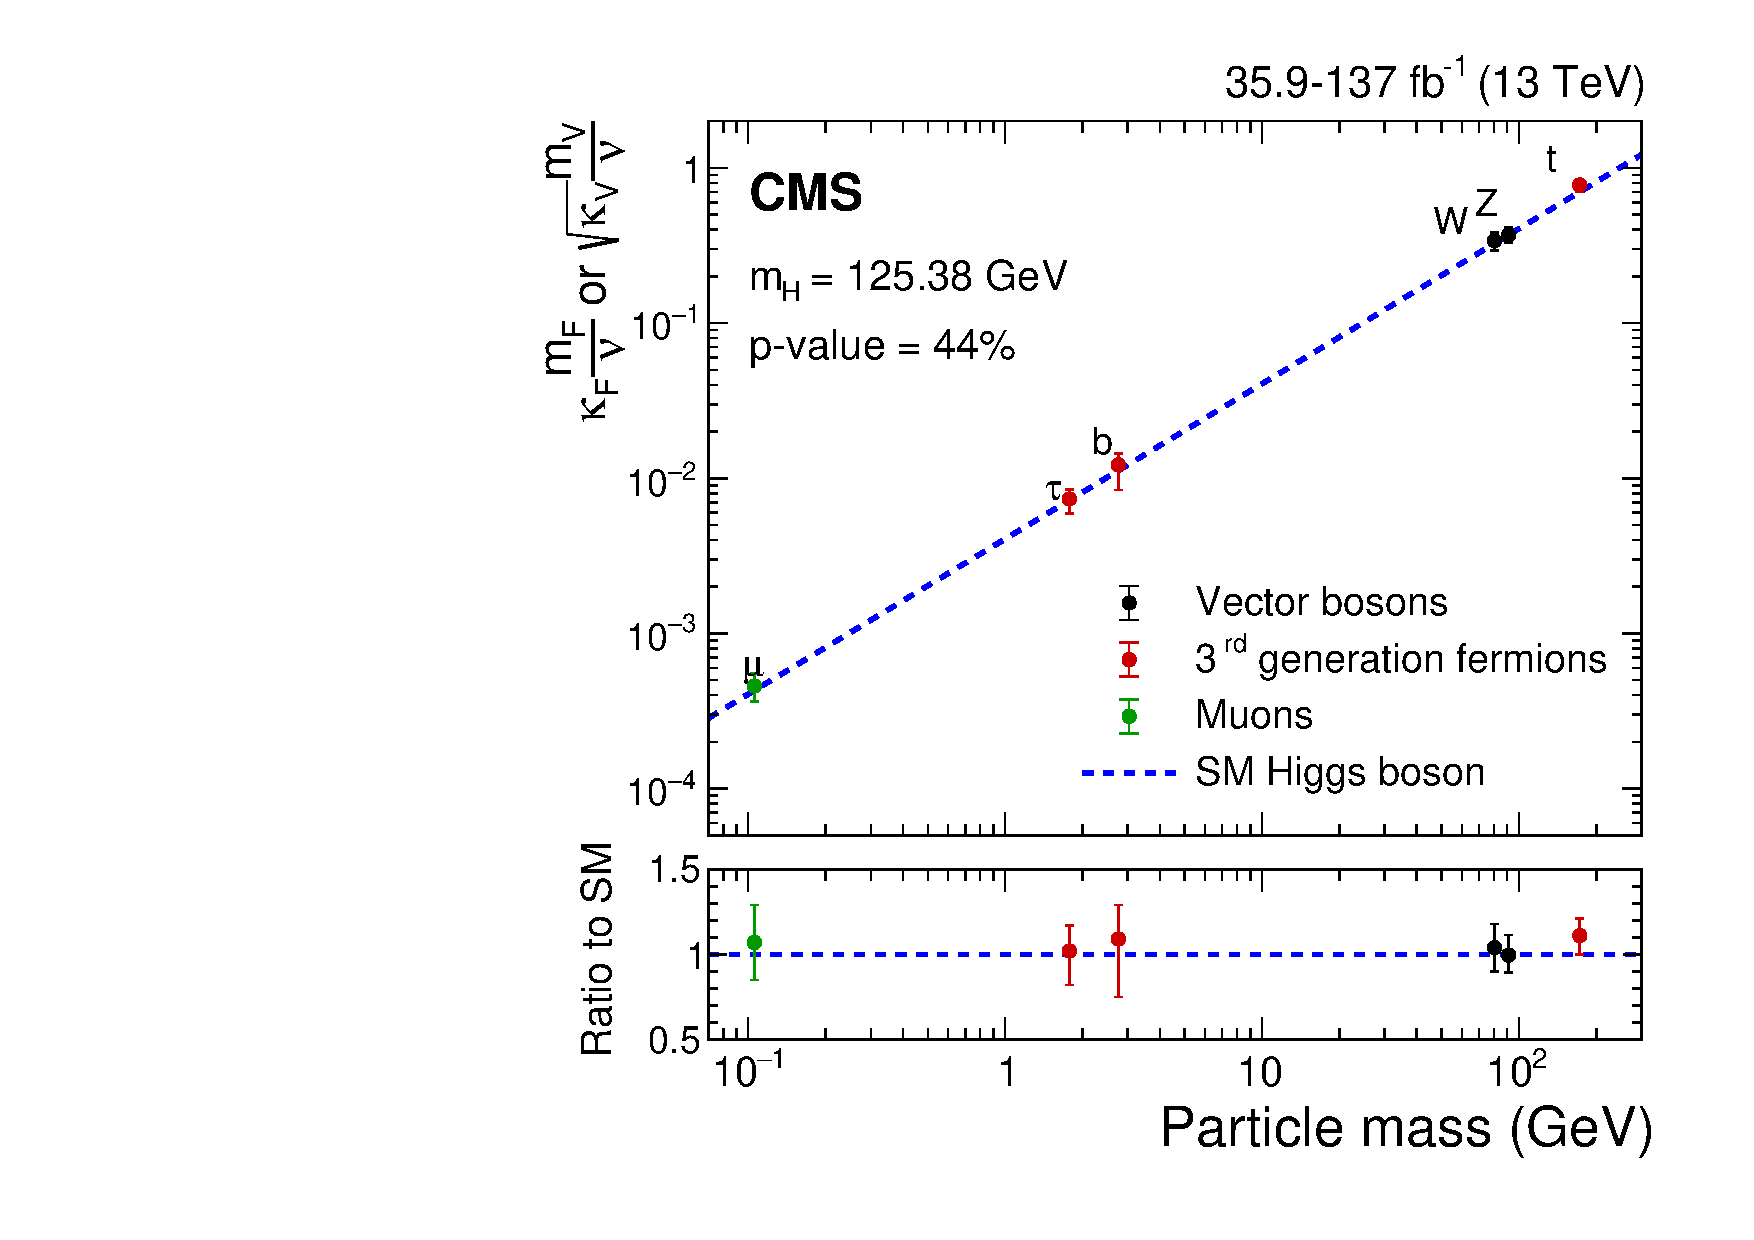
\includegraphics[width=0.45\textwidth]{pics/results/higgs_coupling_new.pdf}
    \caption{Left: A duplicate of Figure~\ref{fig:higgs_2016}, taken from Ref.~\cite{Sirunyan:2640611}. 
             Summary of the CMS measurements on the Higgs coupling to fermions and bosons based on data recorded in 2016.
             Right: The coupling strength measurements updated with this \hmm result. Plot taken from Ref.~\cite{Sirunyan_2021}.}
    \label{fig:higgs_coupling_new}
\end{figure*}

%\section{projection of search at 14 TeV}